%!TEX root = foo-thesis.tex

\chapter{Concept}
\label{chap:concept}

\section{Global Illumination Pipeline Overview}
\label{sec:concept:overview}

\begin{figure}[h]
    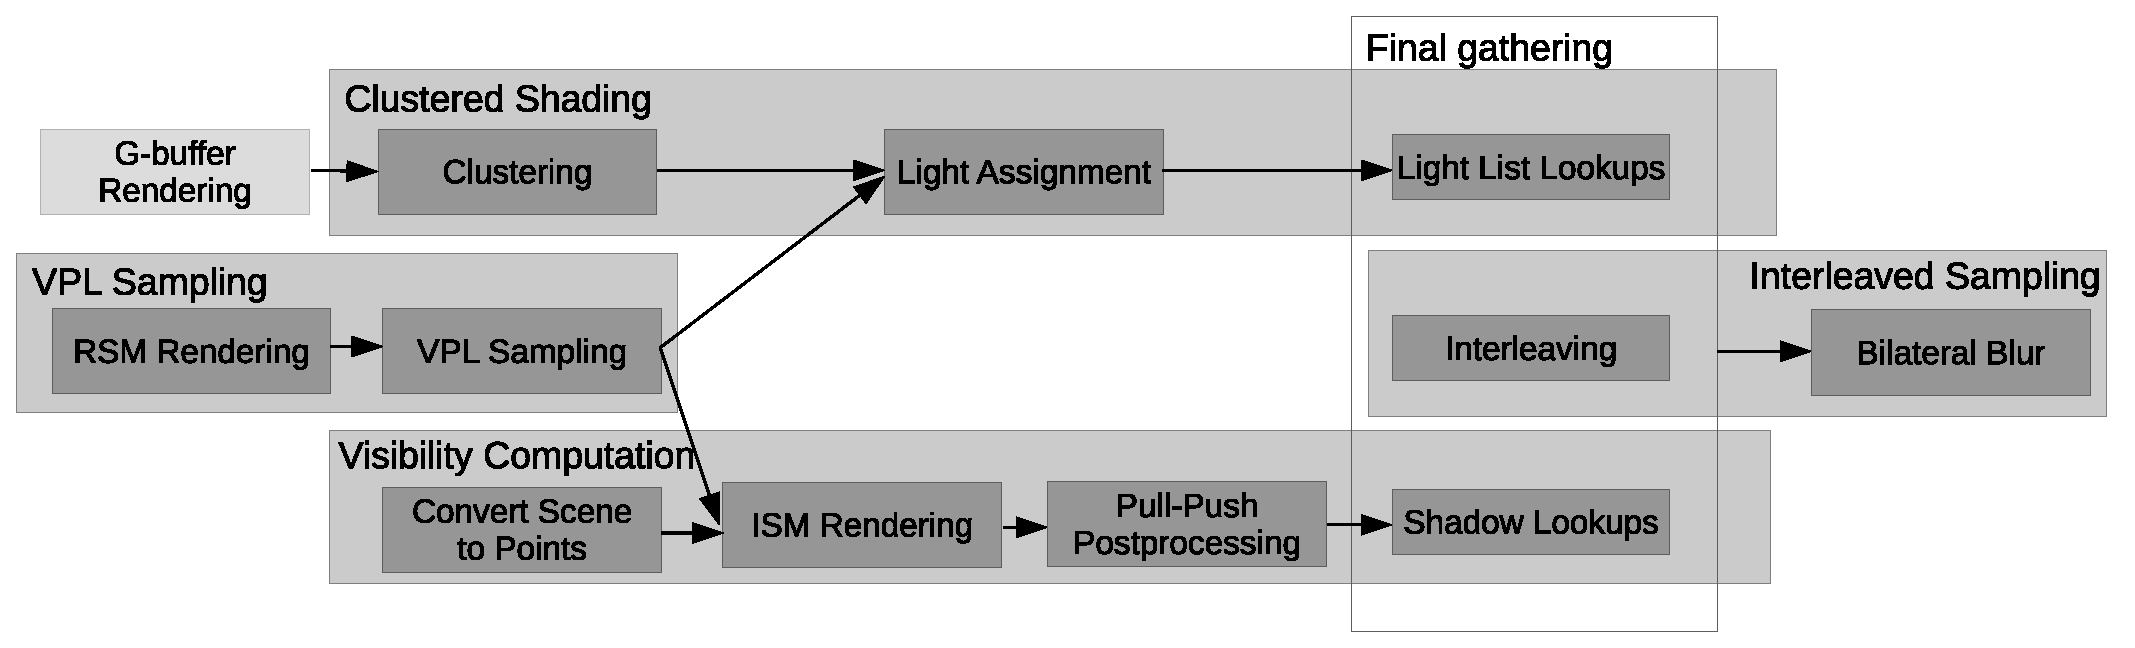
\includegraphics[width=\textwidth]{graphics/GI_pipeline_concept_rough}
    \caption{Global Illumination pipeline concept.}
    \label{fig:GIPipelineConcept}
\end{figure}


This chapter will detail the individual stages of the global illumination pipeline presented in this thesis. Figure~\ref{fig:GIPipelineConcept} provides an overview.
The reflective shadow map and the subsequent VPL sampling (left part of middle row in the diagram) will be covered in the following section.
Section~\ref{sec:concept:ism} describes the rendering process for the imperfect shadow maps (lower row) in detail.
The final gathering step uses data from the clustered shading technique (upper row, detailed in Section~\ref{sec:concept:clusteredShading}) and performs interleaved sampling (right part of middle row, detailed in Section~\ref{sec:concept:interleavedSampling}).
Finally, during final gathering, we use clamping to remove singularities, this is shortly presented in Section~\ref{sec:concept:clamping}.
Our G-buffer rendering does not differ from common deferred rendering pipelines and is not covered further.


\section{Virtual Point Light Sampling with Reflective Shadow Maps}
\label{sec:concept:rsmVplSampling}

VPL sampling has not been the focus of this thesis, therefore we use a rather basic approach by rendering a  simple reflective shadow map and regularly sampling it. \citet{hedman2016sequential} present a more advanced approach.

\begin{outline}
\1 Often preferred due to the simplicity and speed because rasterization. but, first bounce only.

\1 Similar to regular G-Buffer rendering

\1 Like shadowmaps, scene is rendered from the light's viewpoint

\1 Unlike shadowmaps, not only depth is rendered but additionally normal and (diffuse) surface color.

\1 The result can be sampled to create VPLs with a certain position reconstructed from the depth buffer, and normal and color taken from the additional buffers.

\1 In our case, we use regular sampling. Importance-based approaches are available, also the samples can be clustered \cite{} or chosen relative to their estimated contribution to the final output. \citet{hedman2016sequential} uses a different approach without RSMs.

\end{outline}

\section{Visibility Computation with Imperfect Shadow Maps}
\label{sec:concept:ism}


The original paper \citep{ritschel2008ism} converts the scene geometry to a point set in a preprocessing step and uses the points to efficiently render hundreds of shadow maps in parallel. They use splatting to render the points and fill the resulting holes in the shadowmaps with a pull-push algorithm inspired by \citep{Marroquim:2007:reconstruction}.

\citet{ritschel2011ismsViewAdaptive} build on this by converting the scene to a triangle texture dynamically, and sampling the points from that texture. Instead of computing a triangle texture, \citet{barak2013temporally} use the tessellation units of recent GPUs to dynamically convert triangles into points.
We follow this approach since it is relatively simple to implement and inherently dynamic, but have not implemented the adaptive sampling from \citet{ritschel2011ismsViewAdaptive} yet.
\citet{ritschel2008ism} also present multi-bounce indirect illumination with their technique, which we have not implemented.
We describe the point rendering process in the following section and subsequently detail the pull-push algorithm.

\subsection{Point Rendering with Splatting}
\begin{outline}
\1 render the scene
\1 depending on the size of the triangle, set tessellation levels
\1 of the resulting tessellated triangles, take the center, calculate approx world size of disk
\1 while it might be faster to just use the vertices as points, we take the center of each triangle to be more accurate, otherwise the points on the edge of the triangle will enlarge the rendered area considerably.
\1 pick a random VPL, perform culling, render splat into the VPL's ISM. To simplify the calculations, the ISM uses a paraboloid mapping. Here another advantage of the points comes into play: Compared to triangles it is trivial to perform a paraboloid projection for points.
\1 As an optimization, we iterate over several VPLS, and collect some that pass the culling test, and render to those. more in implementation chapter
\1 To remove holes in the resulting shadowmap, the original paper implements a simplified variant of \citet{Marroquim:2007:reconstruction} that only uses depth information from the point rendering. We found that this approach has little benefit over simply enlarging all the point splats during rendering, therefore we did not use it when using splat rendering.
\end{outline}

\subsection{Point Rendering with Pull-Push Postprocessing}

\begin{outline}
\1 Besides point splat rendering, we also pursued a second approach that follows the algorithm of \citet{Marroquim:2007:reconstruction} more closely with the intent to obtain higher-quality shadowmaps. More specifically points are rendered as a single pixel, albeit with additional attributes like size and normal. These are then used in a subsequent reconstruction pass to create an (ideally) hole-free shadowmap. This approach also allowed a point to be rendered into multiple shadowmaps with a moderate performance impact, more on this in the next chapter.

\1 rough overview: the algorithm is a ``pyramid-method'' and uses miplevels.
\1 a pull phase aggregates the information from four pixels of a finer level to one pixel of a coarser level.
\1 a subsequent push phase aggregate four pixels of a coarser level to one pixel of a finer level if the pixel of the finer level contains no data or is determined to belong to an occluded surface. This way, closed surfaces are derived from single-pixel points.

\1 Pull phase
    \2 It only considers pixels that pass the following tests: First, they need to contain a valid depth at all (i.e. a point must have been rendered into this pixel) and second, the pixels depth must not be greater than the frontmost of the four considered pixels plus its depth interval. If this test fails, the point is assumed to belong to a different surface that is occluded and thus should not be used for interpolation.
    \2 The depth interval of each point is determined by adding a constant value to the rendered depth for the points in the lowest miplevel. For interpolated points, the new depth interval spans the calculated depth of the point to the highest depth value of the depth intervals of all points used for aggregation.
    \2 The depth and radius attributes are interpolated in between with equal weights. Since the center of the aggregated point might not match with the position of the pixel (this happens if not all four pixels are used for interpolation), a displacement vector is also calculated that describes the point's location.
\1 Push phase
    \2 Again only pixels that pass certain tests
        \3 Analogous to the pull phase, points must contain a valid depth and not be occluded.
        \3 A radius check: If the pixel's location is outside the point's extends described by the displacement vector and its radius, then the point is not considered either. This is done to limit a point's influence to its actual size.
    \2 The pixel of the finer level might already contain data computed during the pull phase. This data is overwritten if the aggregated data has a smaller depth, i.e. if the original data is considered to be occluded. Otherwise, the original point is left as it is.
    \2 The weights used for interpolation during the push phase are not uniform, see Figure~\ref{fig:???}.
\1 \citet{Marroquim:2007:reconstruction} also use the point's normals to correctly limit the point's size, and \citet{Marroquim:2008:reconstruction2} propose gaussian weights based on the pixel's distance to the point's location, instead constant weights solely based on pixel locations. Both of these additions we have not implemented yet.
\end{outline}



\section{Clustered Deferred Shading}
\label{sec:concept:clusteredShading}

In real-time graphics applications, primarily video games, a technique called \textit{clustered shading} \citep{olsson2012clustered}, has seen increased usage. Its goal is to increase the efficiency of lighting a scene with multiple light sources.
The effectiveness of clustered shading in the context of many-light global illumination has not been studied so far to our knowledge, and we aim to contribute a few datapoints to this end.

The integrated algorithm works as follows:
\begin{outline}
\1 view frustum is divided into a fixed number of clusters
\1 for each fragment, determine cluster. clusters with no fragments are ignored.
\1 for each cluster, determine the VPLs that can reach that cluster, put into light list.
\1 during shading, don't iterate over all VPLs but only those from the light list.
\1 usually, large benefits due to limited radius. we have infinite radius, but at least we can discard half the lights because hemisphere.
\1 As an extension, \citet{olsson2012clustered} propose to calculate explicit bounds for the cluster's fragments to enable more precise culling. we expected only moderate performance gains from that and have not implemented it.
\1 Another extension is to use the surface normal's direction as fourth dimension after the three spatial dimensions for clustering, allowing for some sort of backface culling for even greater efficiency. While this seems more promising in terms of performance gains, we have not implemented it either (wir sind bisher nicht dazu gekommen).
\end{outline}

Clustered shading is an extension and improvement to \textit{tiled shading} \citep{Olsson:2011:TiledShading}, that uses screen-space tiles instead of view-space clusters. Tiled shading has previously combined with many-lights global illumination by \citet{Tokuyoshi:2016:Stochastic}. They use an order of magnitude more lights than we do, but stochastically limit them in range. As a result, the light culling is much more effective in their case.
We implement tiled shading as well and compare it to clustered shading.


\section{Interleaved Sampling}
\label{sec:concept:interleavedSampling}
Interleaved sampling \citep{Keller:2001:InterleavedSampling} is often used to vastly improve the performance impact of GI methods.

\begin{outline}
\1 general idea: given some amount of samples that, in a naïve implementation, would be performed per pixel, distribute those samples over a 4x4 or 8x8 block of pixel
\1 the naïve implementation hurts cache coherency, since adjacent pixels process different samples.
\1 to this end, de-interleaving \citep{segovia2006non} is often used to simultaneously process those pixels that use the same sample set. see Section~\ref{sec:impl:interleavedShading} for details.

\1 results in structured noise and missing information as all pixels have only part of the samples
\1 therefore, geometry-aware blur similar to \citet{laine2007incremental} to distribute the information
\1 the blur is separated (although since it is a bilateral filter, this is mathematically not equivalent, but difference is not noticeable), linear filter, and uses world-space distance and dot product between the samples as weight

\1 all this works because low-frequency effect

\1 In most aspects we follow this standard approach. The only notable deviation is our implementation of de-interleaving that does not use any separate splitting/merging passes, again we defer details to Section~\ref{sec:impl:interleavedShading}.

\end{outline}



\section{Removing Lighting Singularities through Clamping}
\label{sec:concept:clamping}
It's simple, we clamp the singularities. Wouldn't be necessary with infinite number of lights. \citet{hedman2016sequential} reach high accuracy even with clamping and 2k lights.


\todo[color=blue]{textify concept}
